\chapter{Dataset}
\chaptermark{Dataset}
\label{app:dataset}
\graphicspath{{./chapters/Appendix/figs/}}

This appendix shows an overview of the eBDtheque dataset images and their categories.
The corresponding ground truth annotations are described in the next Appendix~\ref{app:groundtruth}.

%TODO: 
\section{Image overview} % (fold)
\label{sec:image_overview}

Figure~\ref{fig:app:1_2} to~\ref{fig:app:9_10} show thumbnails of the eBDtheque dataset images.

%%%%%%%%%%%%%%%%%%%%%%%%%%%%%%%%%%%%%%%%%%%%%%%%%%%
  \begin{figure}[h!]  %trim=l b r t  width=0.5\textwidth,
    \centering
    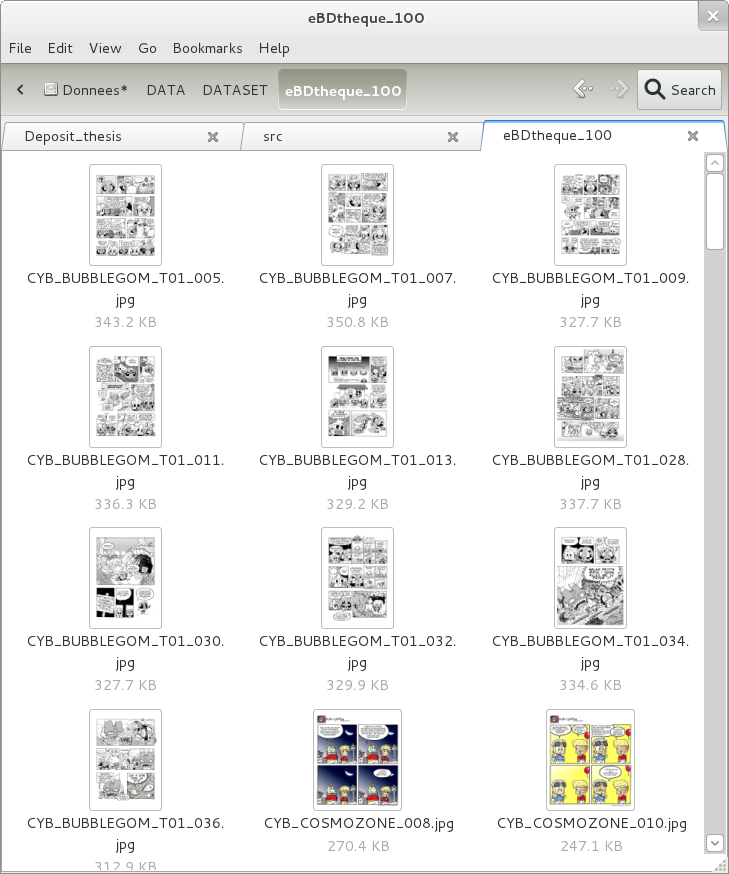
\includegraphics[trim= 5px 10px 30px 152px, clip, width=0.75\textwidth]{thumb_01.png}\\
    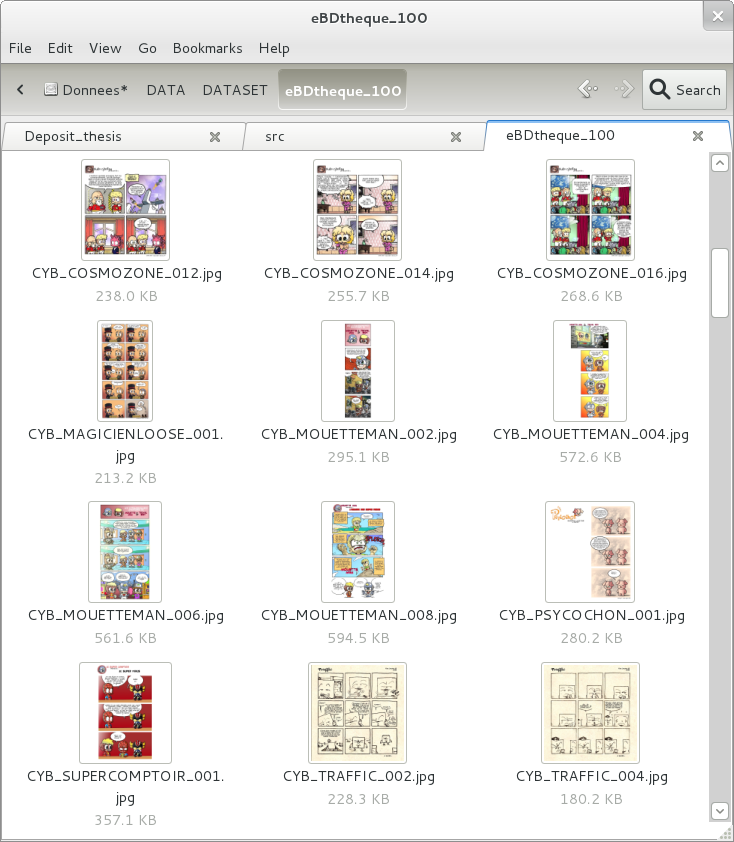
\includegraphics[trim= 5px 10px 30px 152px, clip, width=0.75\textwidth]{thumb_02.png}
    
    \caption{Image group one.}
    \label{fig:app:1_2}
  \end{figure}
  %%%%%%%%%%%%%%%%%%%%%%%%%%%%%%%%%%%%%%%%%%%%%%%%%%%

  %%%%%%%%%%%%%%%%%%%%%%%%%%%%%%%%%%%%%%%%%%%%%%%%%%%
  \begin{figure}[h!]  %trim=l b r t  width=0.5\textwidth,
    \centering
    
    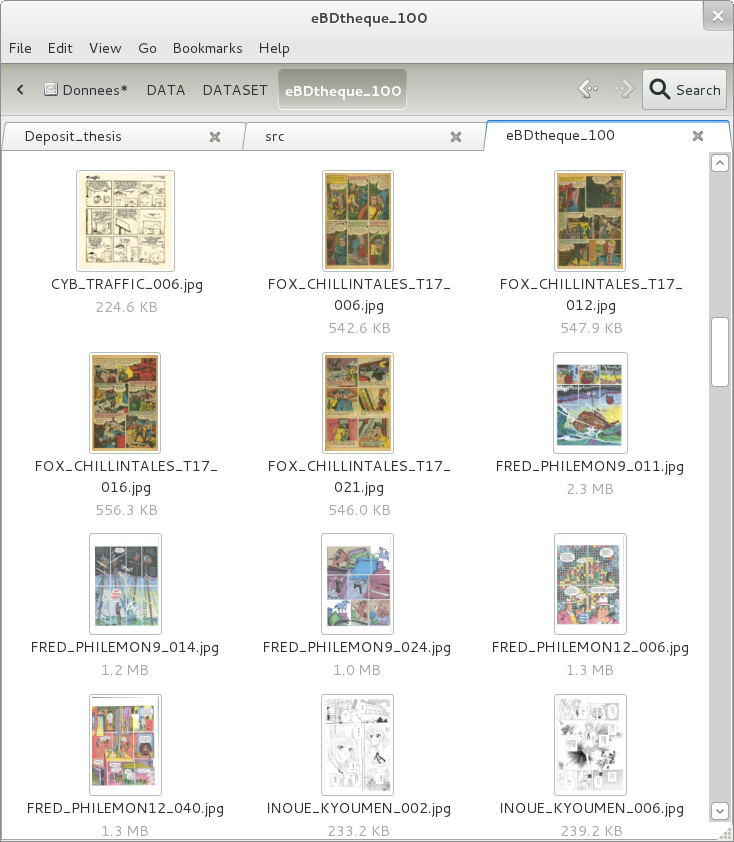
\includegraphics[trim= 5px 10px 30px 152px, clip, width=0.75\textwidth]{thumb_03.png}
    \\
    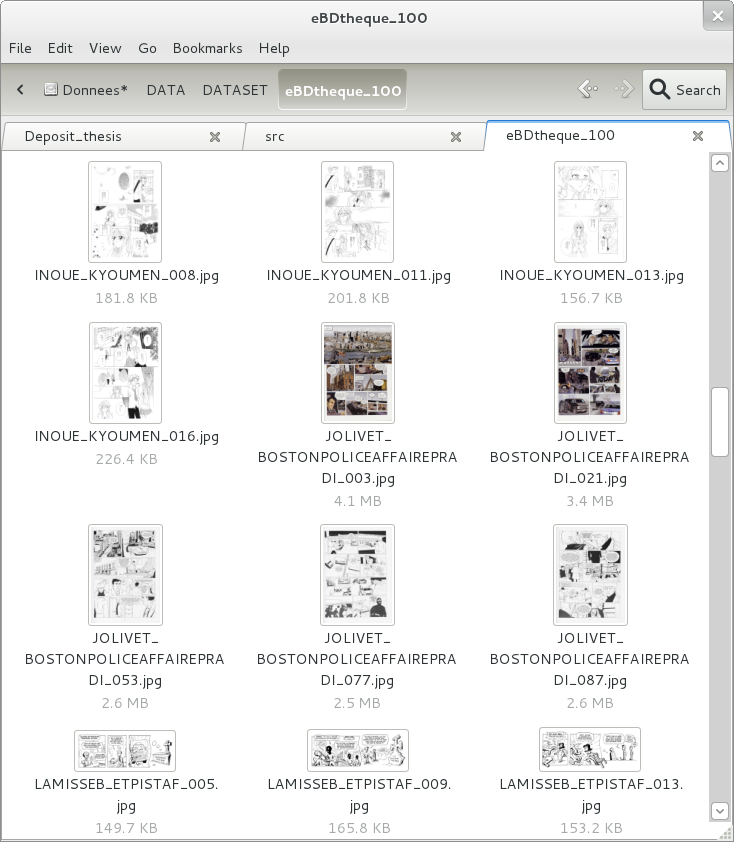
\includegraphics[trim= 5px 10px 30px 152px, clip, width=0.75\textwidth]{thumb_04.png}
    \caption{Image group two}
    \label{fig:app:3_4}
  \end{figure}
  %%%%%%%%%%%%%%%%%%%%%%%%%%%%%%%%%%%%%%%%%%%%%%%%%%%

  %%%%%%%%%%%%%%%%%%%%%%%%%%%%%%%%%%%%%%%%%%%%%%%%%%%
  \begin{figure}[h!]  %trim=l b r t  width=0.5\textwidth,
    \centering
    
    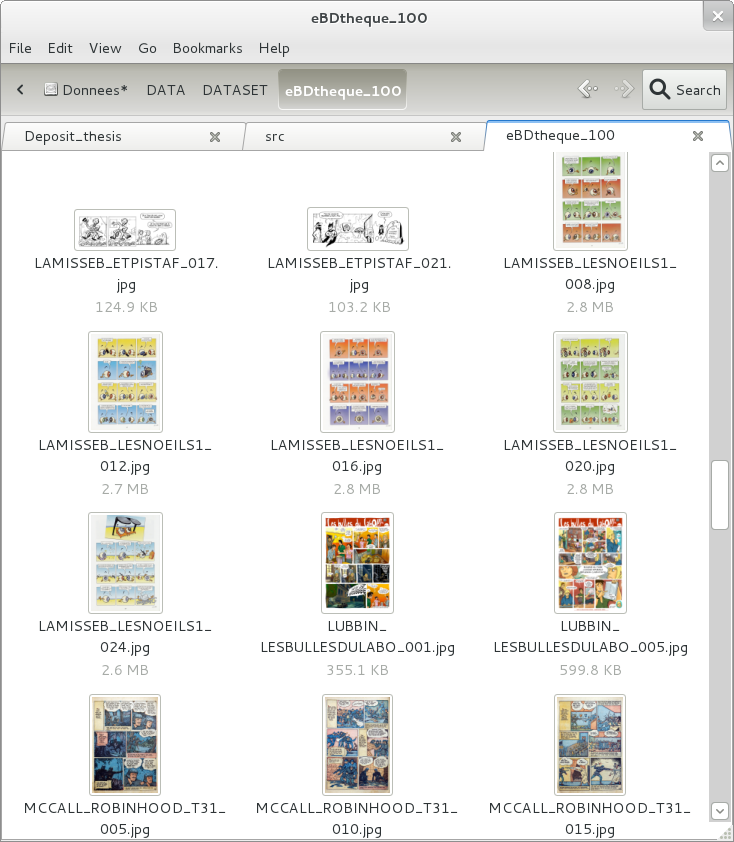
\includegraphics[trim= 5px 10px 30px 152px, clip, width=0.75\textwidth]{thumb_05.png}
    \\
    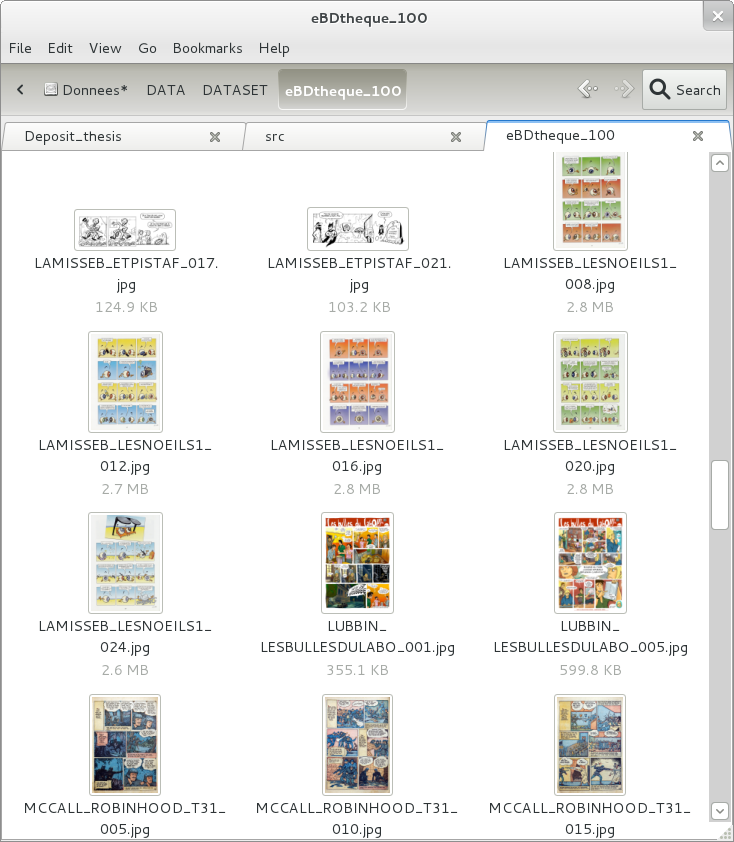
\includegraphics[trim= 5px 10px 30px 152px, clip, width=0.75\textwidth]{thumb_06.png}
    \caption{Image group three.}
    \label{fig:app:5_6}
  \end{figure}
  %%%%%%%%%%%%%%%%%%%%%%%%%%%%%%%%%%%%%%%%%%%%%%%%%%%

  %%%%%%%%%%%%%%%%%%%%%%%%%%%%%%%%%%%%%%%%%%%%%%%%%%%
  \begin{figure}[h!]  %trim=l b r t  width=0.5\textwidth,
    \centering
    
    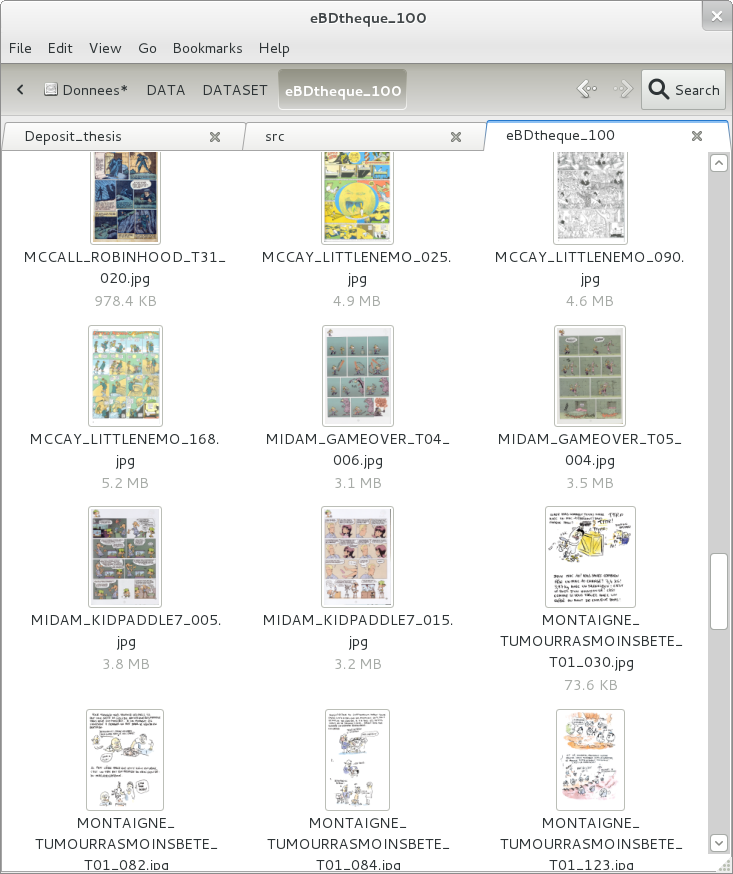
\includegraphics[trim= 5px 10px 30px 152px, clip, width=0.75\textwidth]{thumb_07.png}
    \\
    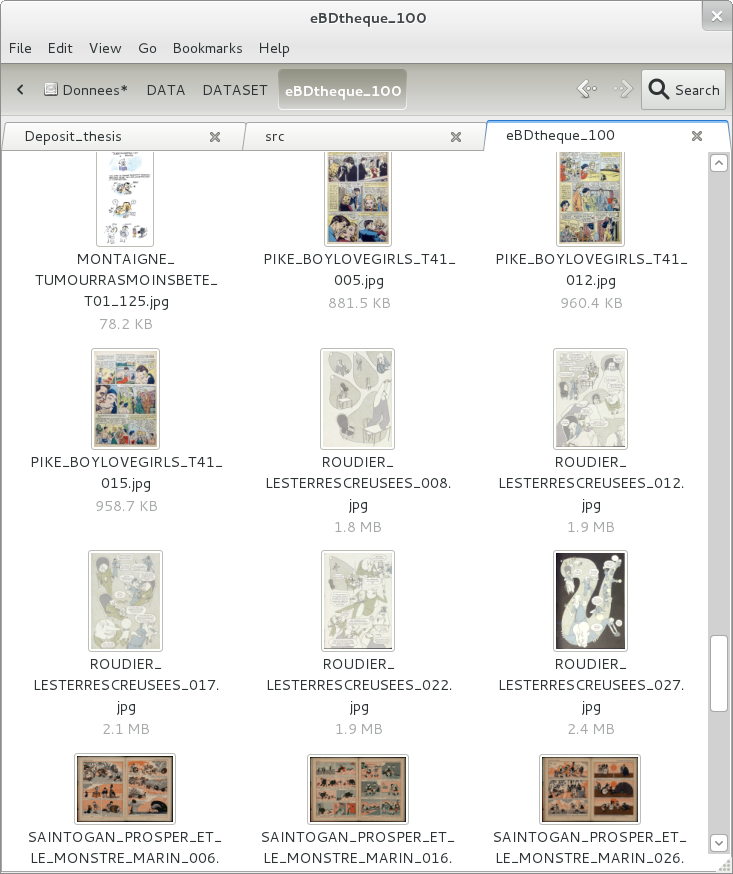
\includegraphics[trim= 5px 10px 30px 152px, clip, width=0.75\textwidth]{thumb_08.png}
    \caption{Image group four.}
    \label{fig:app:7_8}
  \end{figure}
  %%%%%%%%%%%%%%%%%%%%%%%%%%%%%%%%%%%%%%%%%%%%%%%%%%%


  %%%%%%%%%%%%%%%%%%%%%%%%%%%%%%%%%%%%%%%%%%%%%%%%%%%
  \begin{figure}[h!]  %trim=l b r t  width=0.5\textwidth,
    \centering
    
    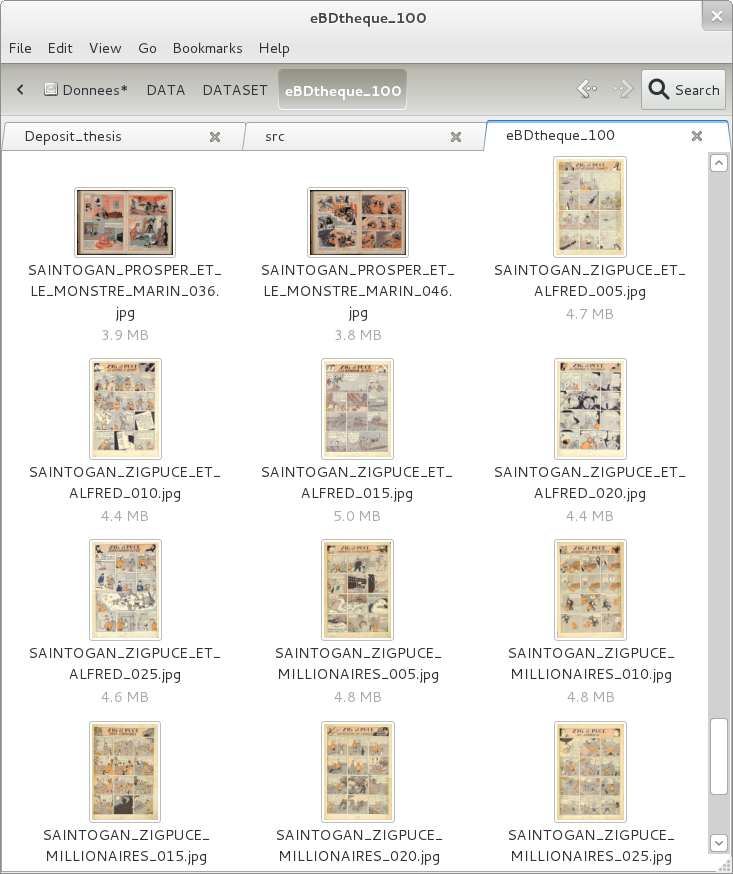
\includegraphics[trim= 5px 10px 30px 152px, clip, width=0.75\textwidth]{thumb_09.png}
    \\
    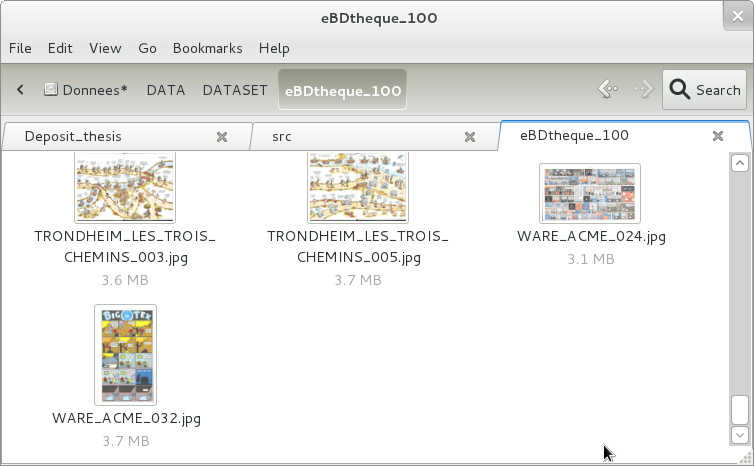
\includegraphics[trim= 5px 10px 30px 152px, clip, width=0.75\textwidth]{thumb_10.png}
    \caption{Image group five.}
    \label{fig:app:9_10}
  \end{figure}
  %%%%%%%%%%%%%%%%%%%%%%%%%%%%%%%%%%%%%%%%%%%%%%%%%%%

% \modif{TODO: display 100 thumbnails with files names on several pages.}
% \modif{TODO: show all dataset thumbnails and file names to understand the evaluation detail bar graphs + give classify into categories (heritage, manga, webcomic, French/English/Japanese)}

% section image_overview (end)

\section{Image categories}

Table~\ref{app:ebdtheque_image_classification} represents the composition of the eBDtheque dataset grouped by categories. 
Corresponding images to the identifiers are available in the previous section and on the dataset website~\footnote{\url{http://ebdtheque.univ-lr.fr/database/?overview=1}}.


\begin{figure}[!ht]
	\begin{center}
	\begin{tabular}{|lllll|}
	\hline
	\textbf{IDs}                              & \textbf{Date} & \textbf{Category}         & \textbf{Colour}     & \textbf{Nb} \\
	\hline
	CYB\_BUBBLEGOM                         & 2009        & French webcomics & Grey & 10       \\
	CYB\_COSMOZONE                         & 2008        & French webcomics & Colour     & 5        \\
	CYB\_MAGICIENLOOSE                     & 2011        & French webcomics & Colour     & 1        \\
	CYB\_MOUETTEMAN                        & 2011        & French webcomics & Colour     & 4        \\
	CYB\_PSYCOCHON                         & 2010        & French webcomics & Colour     & 1        \\
	CYB\_SUPERCOMPTOIR                     & 2011        & French webcomics & Colour     & 1        \\
	CYB\_TRAFFIC                           & 2009        & French webcomics & B\&W       & 3        \\
	FOX\_CHILLINTALES                      & 1953        & American comics  & Colour     & 4        \\
	FRED\_PHILEMON                         & 2004        & French comics    & Colour     & 5        \\
	INOUE\_KYOUMEN                         & 2008        & Japanese manga   & B\&W       & 6        \\
	JOLIVET\_BOSTONPOLICE      & 2010        & French comics    & Colour     & 2        \\
	JOLIVET\_BOSTONPOLICE      & 2010        & French comics    & B\&W       & 3        \\
	LAMISSEB\_ETPISTAF                     & 2012        & French webcomics & B\&W       & 5        \\
	LAMISSEB\_LESNOEILS1                   & 2011        & French comics    & Colour     & 5        \\
	LUBBIN\_LESBULLESDULABO                & 2012        & French webcomics & Colour     & 2        \\
	MCCALL\_ROBINHOOD                      & 1946        & American comics  & Colour     & 4        \\
	MCCAY\_LITTLENEMO                      & 1905        & French comics    & B\&W       & 1        \\
	MCCAY\_LITTLENEMO                      & 1905        & French comics    & Colour     & 2        \\
	MIDAM\_GAMEOVER                        & 2009        & French comics    & Colour     & 2        \\
	MIDAM\_KIDPADDLE                       & 2001        & French comics    & Colour     & 2        \\
	MONTAIGNE\_ \\ TUMOURRASMOINS          & 2011        & French webcomics & Colour     & 5        \\
	PIKE\_BOYLOVEGIRLS                     & 1953        & American comics  & Colour     & 3        \\
	ROUDIER\_ \\ LESTERRESCREUSEES             & 2011        & French comics    & Colour     & 5        \\
	SAINTOGAN\_PROSPER 						& 1934        & French comics    & Colour     & 5        \\
	SAINTOGAN\_ZIGPUCE\_ \\ ET\_ALFRED           & 1952        & French comics    & Colour     & 5        \\
	SAINTOGAN\_ZIGPUCE\_ \\ MILLIONAIRES        & 1928        & French comics    & Colour     & 5        \\
	TRONDHEIM\_ \\ LES\_TROIS\_CHEMINS           & 2000        & French comics    & Colour     & 2        \\
	WARE\_ACME                             & 2005        & American comics  & Colour     & 2        \\
	\hline
	\end{tabular}
\caption[Categories of the images in the eBDtheque dataset]{Categories of the images in the eBDtheque dataset. ``IDs'' column corresponds to the beginning of the image identifier (file name and title of the corresponding grand truth file), ``Date'' is the release date and ``Nb'' the number of image of the category.}
\label{app:ebdtheque_image_classification}
\end{center}
\end{figure}	

% \clearpage
% \newpage
% \section*{Ground truth}
% \label{app:groundtruth}

